\documentclass[english]{elsarticle}
\usepackage[T1]{fontenc}
\usepackage[latin9]{inputenc}
\usepackage{babel}
\usepackage{array}
\usepackage{textcomp}
\usepackage{multirow}
\usepackage{amsmath}
\usepackage{amsthm}
\usepackage{amssymb}
\usepackage{graphicx}
\usepackage[unicode=true]{hyperref}

\makeatletter

%%%%%%%%%%%%%%%%%%%%%%%%%%%%%% LyX specific LaTeX commands.
%% Because html converters don't know tabularnewline
\providecommand{\tabularnewline}{\\}

%%%%%%%%%%%%%%%%%%%%%%%%%%%%%% Textclass specific LaTeX commands.
\theoremstyle{plain}
\newtheorem{thm}{\protect\theoremname}
\theoremstyle{remark}
\newtheorem{rem}[thm]{\protect\remarkname}
\theoremstyle{plain}
\newtheorem{prop}[thm]{\protect\propositionname}
\theoremstyle{definition}
\newtheorem{example}[thm]{\protect\examplename}

\makeatother

\providecommand{\examplename}{Example}
\providecommand{\propositionname}{Proposition}
\providecommand{\remarkname}{Remark}
\providecommand{\theoremname}{Theorem}

\begin{document}
\global\long\def\G{\mathcal{G}}%
\global\long\def\F{\mathcal{F}}%
\global\long\def\var{\mathcal{\mathrm{var}}}%
\global\long\def\E{\mathbb{E}}%
\global\long\def\defined{\stackrel{\text{def}}{=}}%
\global\long\def\Bi{\mathcal{\mathrm{Bi}}}%
\global\long\def\indep#1{{\perp\hspace{-2mm}\perp}#1}%
\global\long\def\P{\mathbb{P}}%
\global\long\def\N{\mathbb{N}}%
\global\long\def\U{\mathbb{U}}%
\global\long\def\E{\mathbb{E}}%
\global\long\def\R{\mathbb{R}}%
\global\long\def\G{\mathcal{G}}%
\global\long\def\g{\mathbb{\Pi}}%
\global\long\def\F{\mathcal{F}}%
\global\long\def\S{\mathcal{S}}%
\global\long\def\Q{\mathcal{Q}}%
\global\long\def\B{\mathcal{B}}%
\global\long\def\ND{\mathcal{N}}%
\global\long\def\XX{\mathcal{X}}%
\global\long\def\indep#1{{\perp\hspace{-2mm}\perp}#1}%
\global\long\def\L{\mathcal{L}}%
\global\long\def\var{\mathrm{var}}%
\global\long\def\cov{\mathrm{cov}}%
\global\long\def\charf{\mathbf{1}}%
\global\long\def\d{\mathrm{d}}%
\global\long\def\M{\mathcal{M}}%
\global\long\def\T{\mathcal{T}}%
\global\long\def\Exp{\mathrm{Exp}}%
\global\long\def\Uniform{\mathrm{U}}%
\global\long\def\eqd{{d\atop =}}%
\global\long\def\A{\mathcal{A}}%
\global\long\def\I{\mathcal{I}}%
\global\long\def\X{\mathcal{X}}%
\global\long\def\supp{\mathrm{support}}%
\global\long\def\H{\mathcal{H}}%
\global\long\def\Z{\mathcal{Z}}%
\global\long\def\as{\qquad a.s.}%
\global\long\def\on{\qquad\text{on }}%
\global\long\def\C{\mathcal{C}}%
\global\long\def\barxi{\overline{\xi}}%
\global\long\def\Po{\mathrm{Po}}%
\global\long\def\barvs{\overline{\varsigma}}%
\global\long\def\bareps{\overline{\varepsilon}}%
\global\long\def\bari{\overline{\iota}}%
\global\long\def\barx{\overline{x}}%
\global\long\def\baru{\overline{u}}%
\global\long\def\bars{\overline{s}}%
\global\long\def\Bi{\mathrm{Bi}}%
\global\long\def\defined{\stackrel{\text{def }}{=}}%
\global\long\def\d{\mathbf{d}}%
\global\long\def\dw{\mathrm{d}}%
\global\long\def\bary{\overline{y}}%
\global\long\def\cvar{\mathrm{CVaR}}%
\global\long\def\barP{P}%
\global\long\def\barX{\overline{X}}%
\global\long\def\barP{\overline{P}}%
\global\long\def\barT{\overline{T}}%
\global\long\def\barB{\overline{B}}%
\global\long\def\barI{\overline{I}}%

\title{SEIR Filter: A Stochastic Model of Epidemics}
\author{Martin \v{S}m\'{\i}d, Lud\v{e}k Berec, Ale\v{s} Anton\'{\i}n Kub\v{e}na, Jan Trnka,
V\'{\i}t Tu\v{c}ek, Milan Zaj\'{\i}\v{c}ek}
\maketitle

\section{Introduction}

Whereas fundamental rationale behind mainstream epidemic models, dating back to the works of Ross (X) and Kermack and McKendrick (X) about a century ago, is relatively easy to comprehend, problems arise when we aim to parameterize such models to data for specific epidemics. The source of troubles is here not only absence of clear and consistent protocols for data collection, but also factors that can never be fully intercepted, such as degrees of compliance in many adopted interventions. This is the case also for COVID-19, despite the somewhat paradoxical observation that we now arguably have the best data on any epidemic in the history. 

Regarding COVID-19, one of the hottest topics has concerned quantifying effects of various non-pharmaceutical interventions (X, X, X). Related to this are then the problems of how effective testing and tracing need be to compensate for an intervention relaxation (X) and how stringent an intervention should be to compensate for a degree of non-compliance potentially related to it (X). Answering these questions, models correctly handling uncertainty are necessary.

Upon construction of realistic models, various data issues have to be coped with, starting from noise (caused both by the epidemic process itself and the data collection), insignificance (difficulty to distinguish impacts of factors from random fluctuations) or co-linearity (difficulty to distinguish two parameters with sufficient certainty); the most severe difficulty, however, is that relevant data (e.g. numbers of infected) are hidden, are observed only indirectly (through the numbers of positive tests, for instance).  Obviously, once any of these phenomena are handled insufficiently, models can provide wrong policy recommendations. 

Mathematical statistics has developed tools to handle these issues. However, to our best knowledge, there is no work systematically doing so for compartmental epidemic models. The goal of this paper is to start filling this gap by proposing a general stochastic epidemic modelling framework. 


Stochastic epidemic models do obviously exist. Apart from agent-based models (X), they are commonly formulated as Poisson processes (X), branching processes (X) or stochastic differential equations (X). However, many of these studies are theoretical, examining their behavior without providing any link to real data and hence an estimation procedure. On the other hand, many other studies use elaborate filtering methods to estimate parameters of their epidemic models, but the models are largely deterministic; statistical models here serve just as tool on the way to understand specific epidemics (X, X, X). Here we in a sense bridge these two approaches, precisely formulating and analyzing a general stochastic epidemic model, discussing its highly practical implications, as well as providing an estimation procedure exemplified on the COVID-19 epidemic in the Czech Republic. Due to practical reasons, we develop our model as discrete in both time and state space. Although applicable to a wide class of epidemic models, we call our framework the SEIR Filter, after a model type most appropriate for the current epidemic of COVID-19.

LUDEK: POssible references 

\cite{farnoosh2017stochastic} diffusion model

 \cite{gibson1998estimating} markov model + plus estimation procedure
together with an estimation procedure is developed. 


We show that contrary to many other fitting methods, our framework enables model parameters to be estimated in a straightforward way, as the exact likelihood (or other estimating) function can be derived, thus allowing faster and more reliable parameter estimation. In addition to the tractability of the estimating function, our model allows for closed form formulas for expected future compartment sizes and the reproduction number. In addition, we provide simple criteria for vanishing and explosion of the epidemic, as well as for bounds that limit expected epidemic sizes given stationary imports. As we demonstrated by stylized examples, many applications of the model are possible, including derivation of implicit formulas regarding compensation measures to intervention relaxation or non-compliance, and of optimal control strategies.

As we have premised, we regard discrete-time discrete-space stochastic
models as the most practical. One of the models closest to our one
is that by \cite{kucharski2020early} (or \cite{prem2020effect}).
When estimating its parameters, the authors use Monte Carlo simulation
to evaluate likelihood functions. We argue and demonstrate that the
parameters of these models can be estimated more straightforward way,
as the likelihood (or other estimating) function can be computed exactly,
allowing for quicker and more reliable estimation.

From the point of mathematical statistics, we model the epidemics (possibly together with some ralated variables) by a partially observed inhomogeneous heteroskedastic vector autoregression process. In line with the usual practice \cite{getz2006modeling}, we assume over-dispersed probability distributions both of the infections and the compartment transitions; thanks to this, we are able to handle realistically not only the actual values of interest, but also the uncertainty associated with them. Moreover, having a standard statistical output of the parameters estimation, we are able to answer questions concerning significance (via P-values), possible co-linearity (via the estimator's correlations) and the hidden compartments values (via the estimate of state-space distribution).

To demonstrate usefulness of our framework, we apply it to the actual COVID-19 pandemic data from the Czech Republic. In particular, we consider four age cohorts, for each of which which we model incidence, admission to- and release from hospitals and deaths. To estimate the model's parameters, we use several partially overlapping datasets; ability to create statistically correct estimates based on such a heterogeneous dataset is, in our opinion, one of the greatest advantages of our approach. We demonstrate both in-sample and out-of-sample prediction ability of our model and, as an example of its possible use, we compare three strategies of vaccination: no vaccination, vaccination without preference and the old-first strategy. 

The paper is organized as follows. After a rigorous probabilistic formulation of the model (Section \ref{sec:Model-Definition}),
we discuss its basic probabilistic properties (Section \ref{sec:Model-Properties}),
its autonomous sub-models and reproduction number (Section \ref{sec:Sub-models-and-Replication})
and asymptotic properties (Section \ref{sec:Asymptotic-behavior}).
Next, we introduce an age-cohort version of the model (Section \ref{sec:cohorts})
and suggest a way of optimal control of the epidemics (Section \ref{sec:oc}).
Further, we discuss estimation of the model (Section \ref{sec:Estimation}).
Next, weand demonstrate its usage by its application to the COVID
pandemics in Czech Republic 2020 (Section \ref{sec:Application-to-The}). Finally, we conclude the paper (Section \ref{sec:Conclusion}).







\section{Model Definition}

\label{sec:Model-Definition}Assume a population of size $s\in\N$,
where $s$ is large. Each individual of the population is either susceptible,
or finds himself in one of the compartments $S_{1},\dots,S_{k}$.
Let $I_{t}\in\N_{0}^{k},$ $t\in\N_{0}^{+},$ be a possibly hidden
external inflow (import) of individuals into the compartments and
let $Z_{t}\in\R^{p},$ $t\in\N_{0}^{+}$, be an observed exogenous
process.

For any $t\in\N_{0}$, let $X_{t}=(X_{t}^{1},\dots,X_{t}^{k})\in\N_{0}^{k},t\in\N_{0},$
be a possibly hidden stochastic process of the compartment sizes which
we define later. Let 
\[
Y_{t}\in\R^{n},\qquad Y_{t}=FX_{t}+\epsilon_{t},\qquad t\in\N_{0},
\]
be a process of observations where $F$ is a deterministic $n\times k$
matrix with rank $n$, and $\epsilon_{t}$ is a random errors vector. 

Denote $(\F_{t})_{t\geq0}$ and $(\G_{t})_{t\geq0}$ the filtrations
induced by $(X,Y,I,Z)$, by $(Y,Z)$, respectively -- these filtrations
may be seen as information flows, $(\F_{t})$ representing all the
information and $(\G_{t})$ the observable one. 

We assume that 
\[
\E(\epsilon_{t+1}|\F_{t})=0,\qquad\var(\epsilon_{t+1}|\F_{t})=\mathrm{diag(}\Gamma_{t}(X_{t},X_{t}^{2})),\qquad t\in\N_{0},
\]
where $\Gamma_{t}$ is a $\G_{t}$-measurable affine linear function
(i.e. $\Gamma_{t}(x,y)=\gamma_{t,0}+\gamma_{t,1}x+\gamma_{t,2}y$
for some $\gamma_{t,0}\in\R^{k}$ and $\gamma_{t,1},\gamma_{t,2}\in\R^{k\times k}$
where all $\gamma_{t,0},\gamma_{t,1}$ and $\gamma_{t,2}$ are $\G_{t}$-measurable). 

We define $X$ recursively: We let $X_{0}$ to be a possibly random
vector and, for any $t\in\N$, we put 
\[
X_{t+1}=I_{t}+N_{t+1}+M_{1,t+1}+\dots+M_{k,t+1}.
\]
Here, $N_{t+1}\in\N_{0}^{k}$ is the inflow of domestically infected
individuals such that $N_{t+1}|\F_{t}\text{\ensuremath{\sim\mathrm{C\Po}(A_{t}X_{t},L)}}$
where $A_{t}=(\alpha_{t}^{ij})_{1\leq i,j\leq k}$, $A_{t}\in\G_{t}$
is a random matrix (the notation $A_{t}\in\G_{t}$ means that $A_{t}$
is a $(\G_{t})$-adapted process) and, for any vector $x$, $\mathrm{CPo}(x,L)$
stands for a vector of independent Compound Poisson variables with
the intensities given by $x$ and the embedded distribution $L$.
Observe that, by basic properties of Compound Poisson distribution,
\[
\frac{\var(N_{t+1}^{i}|\F_{t})}{\E(N_{t+1}^{i}|\F_{t})}=v\defined\frac{\E L^{2}}{\E L}
\]
 (with $\frac{0}{0}\defined\frac{\E L^{2}}{\E L})$, $t\geq0,1\leq i\leq k$.
Further, for any $i$, $M_{i,t+1}\in\N_{0}^{k}$ is the distribution\footnote{Here, we do not mean a probability distribution, but the numbers of
individuals having ended in individual compartments.} of those, who found themselves in compartment $i$ at $t$, between
the compartments at $t+1$. In particular, $M_{i,t+1}^{j}$ (the $j$-th
component of $M_{i,t+1}$) is the number of the individuals who transited
from the compartment $j$ to the compartment $i$ between $t$ to
$t+1$. Further we assume $M_{i,t+1}$, for any $i$, to follow Dirichlet
Multinomial (DM) conditional distribution with parameters $\left(X_{t}^{i},\frac{p_{t}^{1,i}}{c_{i}},\dots,\frac{p_{t}^{k,i}}{c_{i}}\right)$
where $P_{t}=(p_{t}^{ij})_{1\leq i,j\leq k}\in\G_{t}$ is a ``mean''
transition matrix and $(c_{1},\dots,c_{k})$ are deterministic dispersion
parameters. 
\begin{rem}
If we assumed the individuals to change their state according to $P_{t}$
with the transitions being conditionally independent given $\F_{t},$
then we would get $M_{i,t+1}|\F_{t}$ as Multinomial with parameters
$X_{t}^{i}$ and $P_{t}^{(i)}$ where, for any matrix $\Sigma$, $\Sigma^{(i)}$
is its $i$-th column. In practice, however, the assumption of the
conditional independence, is unrealistic, as the course of infection
differs between individuals and (due to mutations) tends to cluster.
The standard way of coping with this situation is using $\mathrm{DM}$
distribution. 
\end{rem}

The flow of individuals between states are illustrated by the following
chart.
\begin{center}
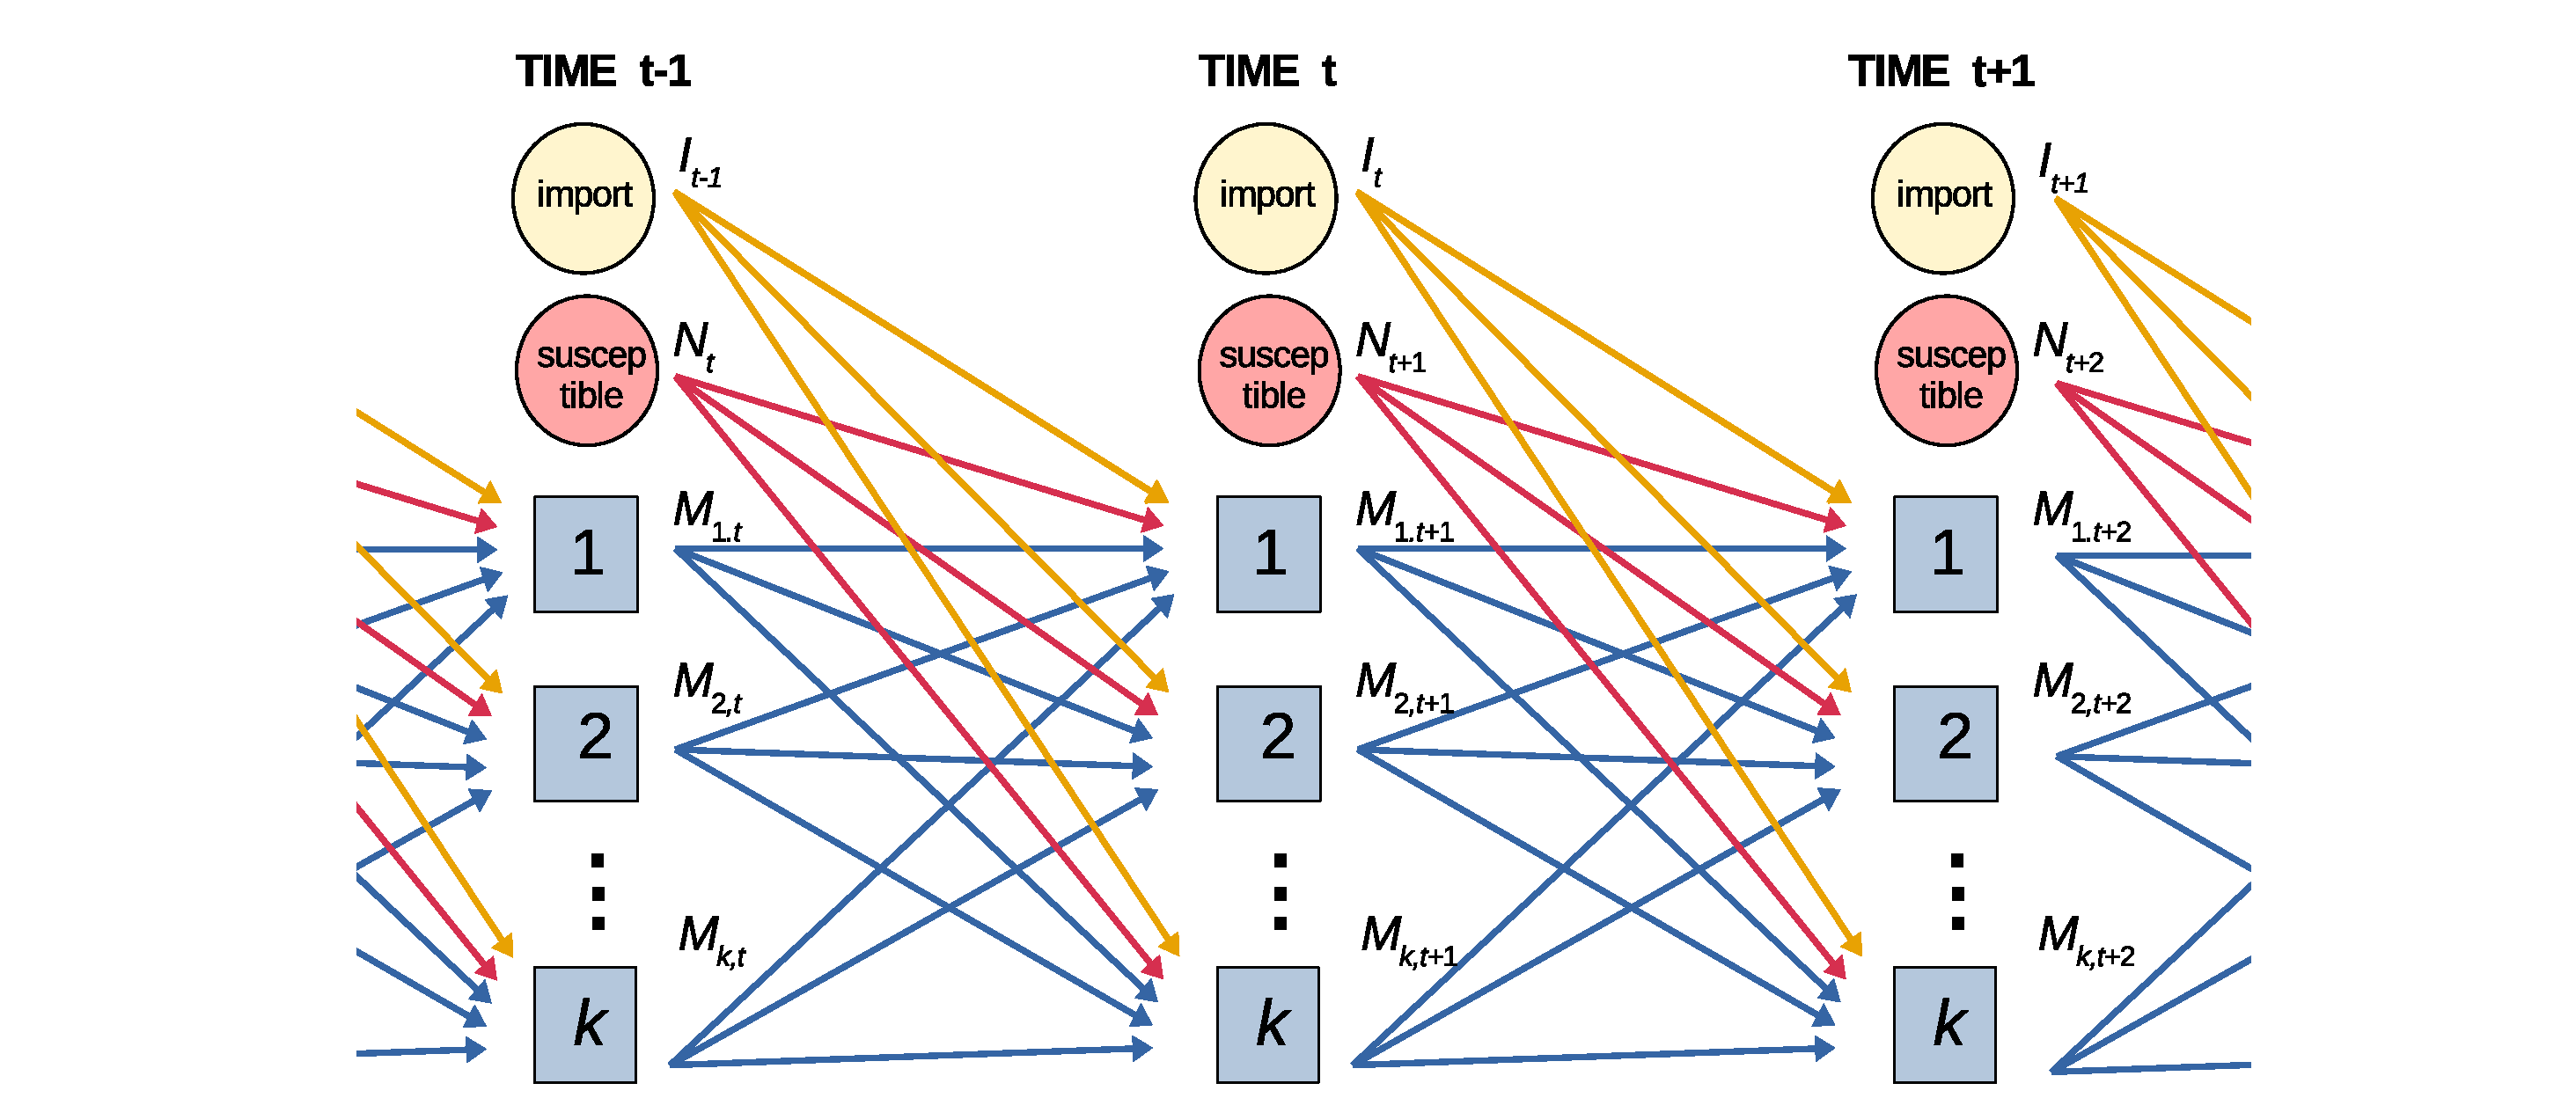
\includegraphics[scale=0.3]{schema}
\par\end{center}

Finally, we assume $N_{t+1},M_{1,t+1},\dots,M_{k,t+1},\epsilon_{t+1}$
to be mutually conditionally independent given $\F_{t}$ (which, in
words, means that all the dependence between the inflows, the transitions
and the observation can be explained by the state of the system at
$t$). Consequently,

\[
\left.X_{t+1}\right|\F_{t}\sim\bigcirc_{1\leq i\leq k}\mathrm{DM}\left(X_{t}^{i},\frac{1}{c_{i}}P_{t}^{(i)}\right)\circ\mathrm{CPo}(A_{t}X_{t},L)\circ\delta(I_{t}),
\]
where $\bigcirc$ and $\circ$ stand for the summation of (mutually)
independent random vectors.

\begin{rem}
The variability of the individual infectiousness may be naturally
reflected by the choice of $L$. To demonstrate it, assume that only
a single compartment (labeled $I$) is infectious, that all the new
infections fall to a single compartment (labeled $E$), and the number
of risk contacts of each infectious individual is Poisson. Let $t\geq0$
and denote $N_{t+1,i}$ the number of the infections, caused by the
$i$-th individual at $t$. 

If the intensity of the contact distribution and the contagion probability
were the same for all, equal to $c$, $p$, respectively, then it
would be $N_{t+1,i}\sim\Po(cq)$, $i\in\N$; consequently, $N_{t+1}^{E}\sim\Po(\lambda X_{t}^{I})$,
$\lambda=cq$, so we may put $\alpha_{t}^{EA}=\lambda$ and $L=\delta_{1}$,
having $\E(N_{t+1}^{E}|\F_{t})=\mathrm{\var}(N_{t+1}^{E}|\F_{t})=\lambda X_{t}$.

Now consider a more realistic situation in which the infectiousness
randomly varies between individuals. A standard way of modeling this
situation is assuming, for each $i$, that the intensity $\lambda_{i}$
of $N_{t+1,i}$ is chosen from Gamma distribution, implying that $N_{t+1,i}$
is negative binomial (see \cite{zhou2013negative}). In particular,
once $\lambda_{i}\sim\Gamma(k,\theta)$, and $N_{t+1,i}|\lambda_{i}=\Po(\lambda_{i})$,
we are getting that $N_{t+1,i}\sim\mathrm{NB}(k,p),$ $p=\frac{\theta}{1+\theta}$,
with
\begin{equation}
\E N_{t+1,i}=\kappa\defined\theta k,\qquad\var(N_{t+1,i})=\kappa v,\qquad v=1+\frac{\kappa}{k}.\label{eq:ev}
\end{equation}
As the Negative Binomial distribution can be represented by a Compound
Poisson one and as the sum of independent Compound Poisson distributions
is Compound Poisson, we have that $N_{t+1}^{E}$ is Compound Poisson\footnote{In particular, $N_{t+1,i}=\mathrm{CPo}(k\ln(1+\theta),\mathrm{Log}(p))$,
where $\mathrm{Log}$ is the Logarithmic distribution, see \cite{zhou2013negative}).
Thus, $N_{t+1}^{E}\sim\mathrm{CPo}(X_{t}^{I}k\ln(1+\theta),\mathrm{Log}(p))$
so we may put $\alpha_{t}^{EA}=k\ln(1+\theta)$, $L=\mathrm{Log}(p)$..} and it follows from (\ref{eq:ev}) that 
\[
\E(N_{t+1}^{E}|\F_{t})=\kappa X_{t},\qquad\mathrm{\var}(N_{t+1}^{E}|\F_{t})=\kappa X_{t}v
\]
\end{rem}

\begin{rem}
\cite{endo2020estimating} claim that the total number $T$ of persons
infected by a single COVID-infectious individual is $T\sim\mathrm{NB}($$K,P)$
where $K\doteq0.1$ and $P$ is such that $\E T=R_{0}$ where $R_{0}$
is the basic reproduction number. As $R_{0}$ of COVID is generally
assumed to be around 2.5 and $\E T=K\frac{P}{1-P}$, it follows that
$P\doteq\frac{25}{26}$. Consequently, the variance-to-mean ratio
is $\tilde{v}\defined\frac{1}{1-P}\doteq26$. Assuming that the individual
is infectious for $f$ days and that his contacts are restricted by
a factor $\beta$, we may, in light of the Compound Poisson reformulation
of $T$, conclude that the number $N_{t+1,i}$ of daily infected is
Compound Poisson with $\E N=\frac{\beta}{f}\E T,\var(N)=\frac{\beta}{f}\var(T)$,
i.e. $N_{t+1,i}$ and consequently $N_{t+1}^{E}$ has the same variance-to-mean
ratio as $T$, i.e. $v=\tilde{v}\doteq26$. 
\end{rem}

\begin{rem}
For any $x\in\N_{0},c\geq0$ and $p\in[0,1]^{k}$ such that $\sum_{i=1}^{k}p^{i}=1$,
we have 
\[
\E\left(\mathrm{DM}(x,\frac{p}{c})\right)=px=\E\left(\mathrm{Multinomial}(x,p)\right)
\]
and 
\[
\var\left(\mathrm{DM}(x,\frac{p}{c})\right)=[\mathrm{diag}(p)-pp^{T}]\frac{x+c}{1+c}x=\var(\mathrm{Multinomial}(x,p))\frac{x+c}{1+c},
\]
from which it is clear that $\mathrm{DM}(x,\frac{p}{c})\rightarrow\mathrm{Multinomial}(x,p)$
as $c\rightarrow\infty$ and that the deviation of the Multinomial
variance matrix grows with decreasing $c$.
\end{rem}


\section{Model Properties}

\label{sec:Model-Properties}By probability calculus, we get that
\begin{multline*}
\E(X_{t+1}|\F_{t})=\E(T_{t}X_{t}+I_{t}|\F_{t})=\E\left(\left.\sum_{i=1}^{k}M_{t+1,i}+N_{t+1}+I_{t}\right|\F_{t}\right)\\
\sum_{i=1}^{k}P_{t}^{(i)}X_{t}^{i}+(\E L)A_{t}X_{t}+I_{t}=T_{t}X_{t}+I_{t},
\end{multline*}
where, for any matrix $\Sigma,$ $\Sigma^{(i)}$ denotes its $i$-th
column, and 
\begin{align}
T_{t} & \defined P_{t}+B_{t},\qquad B_{t}=(\beta_{t}^{i,j})_{1\leq i,j\leq k}\defined(\E L)A_{t},\qquad t\geq0.\label{eq:t}
\end{align}
Consequently, for any $t,s\in\N_{0},t>s$, 
\begin{multline*}
\E(X_{t}|\F_{s})=\E(T_{s,t-1}X_{s}+\sum_{\theta=s}^{t-1}T_{\theta+1,t-1}I_{\theta}|\F_{s})\\
=\E(T_{s,t-1}|\F_{s})X_{s}+\sum_{\theta=s}^{t-1}\E(T_{\theta+1,t-1}I_{\theta}|\F_{s}),
\end{multline*}
where, for any matrix process $\Sigma$, $\Sigma_{s,t}\defined\Sigma_{t}\times\dots\times\Sigma_{s}$
with $\Sigma_{s,s-1}\defined E$ where $E$ is the identity matrix.

In the special case that 
\begin{equation}
B_{\tau}\equiv B_{s},\qquad P_{\tau}\equiv P_{s},\qquad s\leq\tau\leq t,\label{eq:speck}
\end{equation}
 we have 
\[
\E(X_{t}|\F_{s})=T_{s}^{t-s}X_{s}+\sum_{\tau=s}^{t-1}T_{s}^{t-\tau-1}\E(I_{\tau}|\F_{s}),
\]
and 
\[
\E(X_{t}|\G_{s})=T_{s}^{t-s}\E(X_{s}|\G_{s})+\sum_{\tau=s}^{t-1}T_{s}^{t-\tau-1}\E(I_{\theta}|\G_{s})
\]
If, in addition, $\E(I_{\theta}|\G_{s})\equiv\mu$ for some $\mu\in\G_{s}$
and $(E-T_{s})$ is invertible, the latter formula simplifies to
\[
\E(X_{t}|\G_{s})=T_{s}^{t-s}\E(X_{s}|\G_{s})+(E-T_{s})^{-1}(E-T_{s}^{t-s})\mu.
\]
As for variance, we have
\begin{multline*}
\var(X_{t+1}|\F_{t})=\sum_{i=1}^{k}\var(M_{t+1,i}|\F_{t})+\var(N_{t+1}|\F_{t})+\var(I_{t}|\F_{t})\\
=\sum_{1\leq i\leq m}\var\left(\mathrm{DM}\left(X_{t}^{i},\frac{1}{c_{i}}P_{t}^{(i)}\right)\right)+\var(\mathrm{CPo}(A_{t}X_{t},L))+0\\
=\sum_{i\leq t\leq m}\frac{X_{t}^{i}+c_{i}}{1+c_{i}}X_{t}^{i}[\mathrm{diag}(P_{t}^{(i)})-P_{t}^{(i)}(P_{t}^{(i)})^{T}]+\mathrm{diag}(vB_{t}X)\\
=\Lambda_{t}(X_{t},X_{t}^{2})
\end{multline*}
where 
\[
\Lambda_{t}(x,y)\defined\sum_{i=1}^{k}\frac{y^{i}+x^{i}c_{i}}{1+c_{i}}[\mathrm{diag}(P_{t}^{(i)})-P_{t}^{(i)}(P_{t}^{(i)})^{T}]+\mathrm{diag}(vB_{t}x)
\]
(note that $\Lambda_{t}$ is linear in $x,y$). Consequently, 
\begin{equation}
\E\left[\left.{X_{t+1}\atop Y_{t+1}}\right|\F_{t}\right]=\left[{E\atop F}\right](T_{t}X_{t}+I_{t}),\label{eq:mean}
\end{equation}
\[
\var\left(\left.{X_{t+1}\atop Y_{t+1}}\right|\F_{t}\right)=\left[{E\atop F}\right]\Lambda_{t}(X_{t},X_{t}^{2})\left[{E\atop F}\right]^{T}+\mathrm{diag}\left({0_{k}\atop \Gamma_{t}(X_{t},X_{t}^{2})}\right),\qquad t\geq0.
\]



\section{Sub-epidemics and Reproduction Number}

\label{sec:Sub-models-and-Replication}We say that the subset of compartments
$D=\{s_{1},\dots,s_{m}\}$ is $subepidemic$ if, for any $t$ and
any $i\in D$ and $j\notin D$, $\beta_{t}^{ij}\equiv\beta^{ji}\equiv0$,
and $p_{t}^{ij}\equiv0$. In words this means that, for any $i\in D$,
the $i$-th compartment does not increase through direct infection,
the infection does not depend on the compartment, and it is impossible
to get to the state $i$ once being outside $D$.

Let, after a possible re-ordering, $m\in\N$ be such that $\{1,\dots,m\}$
is subepidemic (such $m$ always exists because it can be always put
to $k$). For any vector $x\in\R^{k}$, denote $\overline{x}$ its
restriction to $(1,\dots,m)$ and, for any matrix $A\in\R^{k\times k}$,
denote $\overline{A}$ its restriction to $(1,\dots,m)\times(1,\dots,m)$.

Observe that $\barX$ follows a slightly modified version of our model,
namely 
\[
\left.\barX_{t+1}\right|\F_{t}\sim\bigcirc_{1\leq i\leq m}\mathrm{DM}^{-}(\barX_{t}^{i},\frac{1}{c}\barP_{t}^{(i)},c)\circ\mathrm{CPo}(\barB_{t}\barX_{t},L)\circ\delta(\barI_{t}).
\]
where, for any $x\in\N_{0},\alpha\in\R_{+}^{m}$ and $c>0$, $\mathrm{DM}^{-}(x,\alpha,c)$
is the marginal distribution of the first $m$ components of $\mathrm{DM}\left(x,\left[{\alpha\atop c-\sum_{i=1}^{m}\alpha^{i}}\right]\right)$.
(by the aggregation property of $\mathrm{DM}$).

For any $t$, we define the reproduction number $r_{t}$ (of a subepidemic
$\{1,\dots,m\}$) as 
\[
r_{t}\defined\sum_{\tau=t}^{\infty}\mathbf{1}^{T}\E(B_{\tau}\barP_{t,\tau-1}|\F_{t-1})\pi_{t},\qquad\pi_{t}=\E\left\{ \left.\nu\left(\overline{N}_{t}+\overline{I}_{t-1}\right)\right|\F_{t-1}\right\} .
\]
where $\nu$ is unit normalization of a vector. Observe that $r_{t}$
complies with the usual definition of reproduction number as it equals
to the conditional expectation (w.r.t. $\F_{t-1})$ of the infections
caused by an individual having arrived at $t$. To see it, note that
$\pi_{t}$ is the conditional distribution of the state in which a
randomly chosen newcomer (the one brought by the import or by the
infection) finds himself at $t$, and observe that, for each newcomer
at $t$, the expected number of those infected by him at $t+1$ is
given by the sum of the components of $\barB{}_{t}\pi_{t}$, the expected
number infected at $t+1$ is given by the sum of components of $\barB_{t+1}\barP_{t}\pi_{t}$
etc.

If $\F_{t}\neq\G_{t}$ (i.e. $X$ is not fully observed), then the
reproduction number has to be estimated, most naturally by its conditional
expectation with respect to the known information: 
\[
\tilde{r}_{t}\defined\E(r_{t}|\G_{t})=\sum_{\tau=t}^{\infty}\mathbf{1}^{T}\E(\barB_{\tau}\barP_{t,\tau-1}\pi_{t}|\G_{t-1}).
\]
In the special case of $\barB_{\tau}\equiv\barB_{t-1},\barP_{\tau}\equiv\barP_{t-1}$,
$\tau\geq t$, with $\rho(\barP_{t-1})<1$ where $\rho$ is the spectral
radius, the formula simplifies to
\[
\tilde{r}_{t}=\mathbf{1}^{T}\barB_{t-1}\left(\sum_{i=0}^{\infty}\barP_{t-1}^{i}\right)\E(\pi_{t}|\G_{t-1})=\mathbf{1}^{T}\barB_{t-1}(E-\barP_{t-1})^{-1}\E(\pi_{t}|\G_{t-1}).
\]
Note that, once $\overline{N}$ and/or $\overline{I}$ are possibly
not observed, there could be difficulties computing $\E(\pi_{t}|\G_{t-1})$
-- yet the estimate $\E(\pi_{t}|\G_{t-1})\doteq\nu(\barB_{t-1}\E(\barX_{t-1}|\G_{t-1})+\E(\barI_{t-1}|\G_{t-1}))$
seems a straightforward choice, it is generally not unbiased due to
the normalization. This problem, however, vanishes if the imports
and new infections all fall into a single state (typically called
exposed and labeled $E$), in which case $\pi_{t}\equiv(1,0,\dots,0)^{T}$.



\section{Asymptotic Behavior}

\label{sec:Asymptotic-behavior}Keep assuming that $\{1,\dots,m\}$
is subepidemic. The next Proposition states conditions for vanishing,
explosion and ``stationary'' behavior of the subepidemic.
\begin{prop}
\label{prop:as}(i) If $\barT_{t}\leq S$ component-wise, where S
is deterministic with $\sigma\defined\rho(S)<1,$ and if $\E\barI_{t}=o(t^{-\alpha})$
for some $\alpha>0$, then $\barX_{t}\rightarrow0$ almost sure. Here,
$\rho$ denotes the spectral radius of a matrix.\\
(ii) If $\barT_{t}\geq R$ where R is deterministic irreducible with
$\varrho\defined\rho(R)>1$ and either $\E\barX_{0}\neq0$ or $\E\barI_{\tau}\neq0$
for some $\tau$, then $\|\E\barX_{t}\|\rightarrow\infty$.\\
(iii) If $\E\barI_{t}\equiv\mu$ for some $\text{\ensuremath{\mu} }$and
$R\leq\barT_{t}\leq S$ such that $\sigma\defined\rho(S)<1,$ then
\[
\liminf_{t}\E\barI_{t}\ge(E-R)^{-1}\mu,\qquad\limsup_{t}\E\barI_{t}\leq(E-S)^{-1}\mu
\]
\end{prop}

\begin{proof}
(i) We have 
\begin{multline*}
\E\barX_{t}=\E(\E(\barX_{t}|\G_{0}))=\E(\barT_{0,\tau-1}X_{0}+\sum_{\theta=0}^{t-1}\barT_{\theta+1,t-1}\E(\barI_{\theta}|\G_{0}))\\
\leq\E(S^{t}X_{0}+\sum_{\theta=0}^{t-1}S^{t-\theta-1}\E(\barI_{\theta}|\G_{0}))\leq a_{t}+b_{t,}\qquad a_{t}=S^{t}\E\barX_{0},\qquad b_{t}=\sum_{\theta=0}^{t-1}S^{t-\theta-1}\E\barI_{\theta}
\end{multline*}
Thanks to the sub-unit spectral radius of $S$, we have $a_{t}\rightarrow0$.
Further, by the non-negativity of $H$ and the properties of convergence,
there exists $c\in\R_{+}^{m}$ such that $\E\barI_{t}\leq c(t+1)^{-1}.$
Thus, for any $\varsigma$ fulfilling $\sigma<\varsigma<1$, we get,
after re-indexing the sum, 
\[
b_{t}=\sum_{\tau=0}^{t-1}S^{\tau}\E\barI_{t-\tau-1}\leq\sum_{\tau=0}^{t-1}S^{\tau}c\frac{1}{(t-\tau)^{\alpha}}=\underbrace{\frac{1}{t^{\alpha}}}_{\rightarrow0}\times\underbrace{\sum_{\tau=0}^{t-1}(\varsigma^{-1}S)^{\tau}c}_{\rightarrow(E-\varsigma^{-1}S)^{-1}c}\underbrace{\left(\frac{\varsigma^{\tau/\alpha}}{t-\tau}\right)^{\alpha}}_{\leq d}\rightarrow0;
\]
the second convergence holding because $\rho(\varsigma^{-1}S)=\frac{\sigma}{\varsigma_{t}}<1$,
the upper bound $d$ existing as $f(\tau)\defined\frac{t\varsigma^{\tau/\alpha}}{t-\tau}$
increases in $\tau=t-1$ and its derivative has only a single root,
so we have $f(\tau)\leq\max(f(0),f(t-1))=\max(1,\varsigma^{\frac{t-1}{\alpha}}t)\leq d\defined\max(1,\frac{1}{e\varsigma^{1/\alpha}|\alpha^{-1}\ln\varsigma|})$
on $[0,t-1].$ Finally, thanks to the non-negativity of $\barX,$
convergence of $\E\barX_{t}$ suffices for a.s. convergence of $\barX_{t}$.

(ii) Let $\E\barX_{0}\neq0$ and $\varrho>1$. As $R$ is irreducible
non-negative $\varrho$ is its eigenvalue and the corresponding eigenvector
$x$ is positive by the Perron-Frobenius Theorem. Further, by the
irreducibility of $T$, there exists $n$ such that $y\defined R^{n}\E\barX_{0}>0$
component-wise, so there exist $e>0$ such that $y\geq ex$. Thus
\[
\E\barX_{t}\geq R^{t}\E\barX_{0}\geq R^{t-n}y\geq eR^{t-n}x
\]
norm of which converges to infinity. The proof for $\E\barI_{\tau}\neq0$
is analogous.

(iii)

\begin{multline*}
\E\barX_{t}
=\sum_{\tau=0}^{t-1}\barT_{\tau,t-2}\mu+\barT_{0,t-1}\E\barX_{0}\leq\sum_{\tau=0}^{t-1}
S^{\tau}\mu+S^{t-1}\E\barX_{0}
\rightarrow (\sum_{\tau=0}^{\infty}S^{\tau}) 
\mu
$
$
=(E-S)^{-1}
\mu
\end{multline*}
and similarly for $R.$

\end{proof}


\begin{example}
\label{exa:e1}Say there are five states $E$ -- exposed, $I_{a}$
-- infectious asymptomatic, who will never show symptoms, $I_{p}$
-- infectious pre-symptomatic, who will later show symptoms, $I_{s}$
-- infectious symptomatic, and $R$ -- removed, which includes the
recovered, the dead, and the infectious isolated. We index the states
by $e,a,p,s,r$. For simplicity we assume $v=1$ which means that
the new infections are Poisson rather than Compound Poisson. All the
infectious states are equally infectious, i.e. $\beta_{t}^{ex}=\beta_{t}$,
$x\in\{a,p,s\},$ where $\beta$ is a $\G_{t}$-adapted process. The
probability that the exposed transits to $\{a,p\}$ is $\sigma,$
the probability of completely asymptomatic course is $\alpha$, the
probability of transition from $I_{p}$ to $I_{s}$ is $\varsigma$.
Further, the probability of ending $I_{a}$ or $I_{s}$, by natural
causes (recovery, end of infectiousness, death in case of $I_{s}$)
is $\varrho_{a}$, $\varrho_{s}$, respectively. Finally, the probability
that a symptomatic individual isolates himself is $\eta$ and the
probability that the individual finding herself in state $i$ is isolated
is $\theta_{t}^{i}$ for some $\G_{t}$-adapted process $\theta^{i}$.
The situation is illustrated on the following Figure: 
\begin{center}
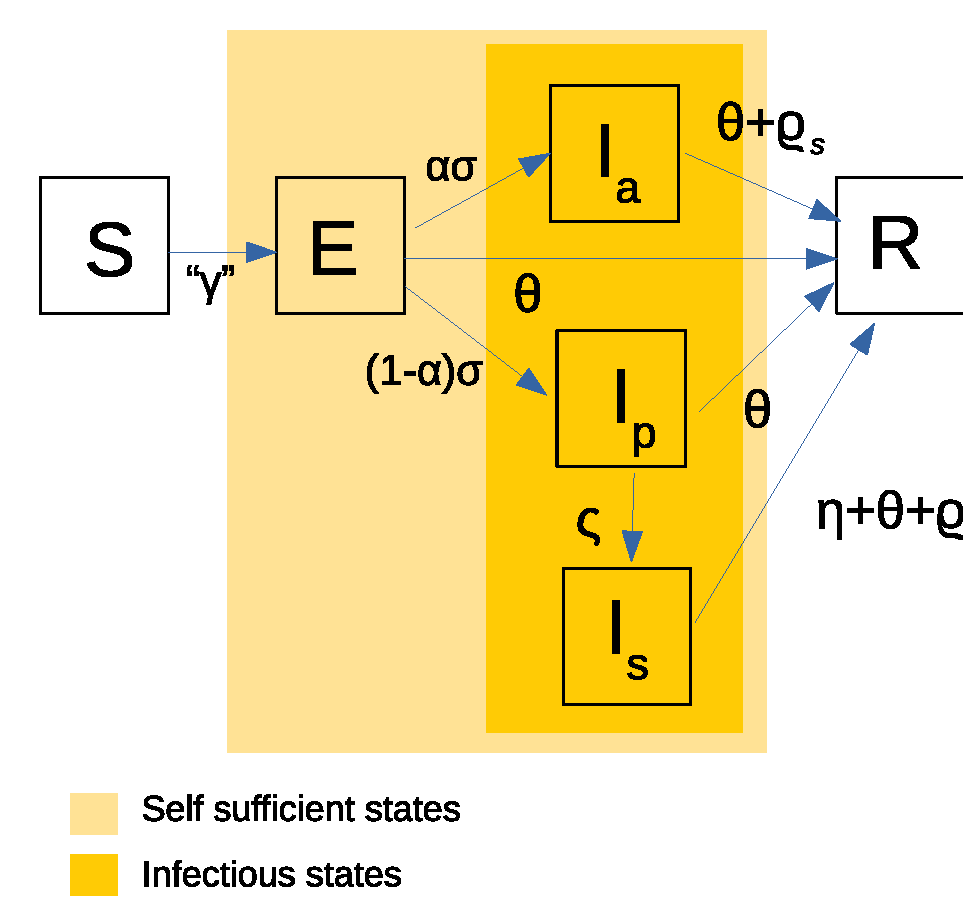
\includegraphics[scale=0.3]{simple}
\par\end{center}

If we neglect (small) joint probabilities of natural exits from the
infectious states and the isolations, we get 
\[
P_{t}=\left[\begin{array}{ccccc}
1-\sigma-\theta_{t}^{e} & 0 & 0 & 0 & 0\\
\alpha\sigma & 1-\varrho_{a}-\theta_{t}^{a} & 0 & 0 & 0\\
(1-\alpha)\sigma & 0 & 1-\varsigma-\theta_{t}^{p} & 0 & 0\\
0 & 0 & \varsigma & 1-\varrho_{s}-\eta-\theta_{t}^{s} & 0\\
\theta_{t}^{e} & \theta_{t}^{a}+\varrho_{a} & \theta_{t}^{p} & \theta_{t}^{s}+\eta+\varrho_{s} & 1
\end{array}\right],\qquad B_{t}=\left[\begin{array}{ccccc}
0 & \beta_{t} & \beta_{t} & \beta_{t} & 0\\
0 & 0 & 0 & 0 & 0\\
0 & 0 & 0 & 0 & 0\\
0 & 0 & 0 & 0 & 0\\
0 & 0 & 0 & 0 & 0
\end{array}\right]
\]
Clearly, we can put $m=4$ (the first four states form a sub-epidemic),
getting 
\[
\barT_{t}=Q+\beta_{t}C-\mathrm{diag}(\theta_{t}),\qquad Q=\left[\begin{array}{cccc}
1-\sigma & 0 & 0 & 0\\
\alpha\sigma & 1-\varrho_{a} & 0 & 0\\
(1-\alpha)\sigma & 0 & 1-\varsigma & 0\\
0 & 0 & \varsigma & 1-\varrho_{s}-\eta
\end{array}\right],\qquad C=\left[\begin{array}{cccc}
0 & 1 & 1 & 1\\
0 & 0 & 0 & 0\\
0 & 0 & 0 & 0\\
0 & 0 & 0 & 0
\end{array}\right]..
\]
Further we assume $\theta_{t}\defined\theta_{t}^{e}=\theta_{t}^{a}=\theta_{t}^{p}=\theta_{t}^{s}$,
which yields, by the well known rule, $\rho(\barT_{t})=\rho(Q+\beta_{t}C)-\theta_{t}$.
We consider two ways of decreasing the spectral radius: decreasing
the infection rate $\beta_{t}$ (typically by wide counter-epidemic
measures) and increasing the isolation rate $\theta_{t}$ (e.g. by
strengthening the testing and tracing capacity).

Once there is a ``target'' spectral radius $\rho_{0},$ all the
combinations of $\beta$ and $\theta$ yielding $\rho(\barT_{t})=\rho_{0}$
fulfill $\rho_{0}+\theta-\rho(Q+\beta_{t}C)=0,$which gives a ``marginal
rate of substitiution'' $\theta(\beta)'=-\frac{\partial}{\partial\beta}\rho(Q+\beta_{t}C)$
of the infectiousness by the isolation, i.e. how much we have to increase
the isolation speed when we release the restrictions.
\end{example}

\begin{example}
Assume there is a fraction $\nu$ of the population is non-compliant,
which means that, once a restriction on social contacts is imposed,
they apply it only partially. Assume that, without restrictions, the
population is mixed which means that each individual, compliant or
not, has, up to a constant, $(1-\nu)$ contacts with the compliant
individuals and $\nu$ contacts with the non-compliant ones. Once
there is a measure imposed under which the compliant individuals restrict
their opportunities to contacts by $\phi$, the non-compliant ones
do so only to $f(\phi)>\phi$ . As a result, the compliant ones will
have, up to a constant, $\phi^{2}(1-\nu)$ contacts with the compliant
ones, $\phi f(\phi)\nu$ contacts with the non-compliant ones, while
the non-compliant will have $\phi f(\phi)(1-\nu)$ and $f(\phi)^{2}\nu$
contacts with the compliant, non-compliant, respectively.

Assuming a simple epidemic model with compartments $I_{c}$ - infected
compliant, $I_{n}$ - infected non-compliant, and $R$ - removed,
with the course of infection being the same for both the compartments
such that $\beta_{t}^{1i}=\beta c_{i}$, $i\in\{1,2\},$ where $\beta$
is a constant and $c_{i}$ is the number of contacts of the $i$-th
sub-population, this gives 
\[
P_{t}=\left[\begin{array}{ccc}
1-\varrho & 0 & 0\\
0 & 1-\varrho & 0\\
\varrho & \varrho & 1
\end{array}\right],\qquad B_{t}=\left[\begin{array}{ccc}
\beta\phi^{2}(1-\nu) & \,\beta\phi f(\phi)\nu\, & 0\\
\beta\phi f(\phi)(1-\nu) & \,\beta f(\phi)^{2}\nu\, & 0\\
0 & 0 & 1
\end{array}\right]
\]
where $\varrho$ is a removal rate (perhaps consisting of an artificial
and a natural part). This gives 
\[
\barT_{t}=\beta C+(1-\varrho)E,\qquad C=\left[\begin{array}{cc}
\phi^{2}(1-\nu) & \,\phi f(\phi)\nu\\
\phi f(\phi)(1-\nu) & \,f(\phi)^{2}\nu
\end{array}\right]
\]
with 
\[
\varrho(\barT_{t})=\beta\rho(C)+(1-\varrho).
\]
As the characteristic polynomial of $C$ is 
\[
\lambda^{2}-\lambda g,\qquad g=g(\phi,\nu)=\phi^{2}(1-\nu)+f(\phi)^{2}\nu
\]
we clearly have $\rho(C)=g.$

Now say that our goal is to decrease $\rho(\barT_{t})$ to a predetermined
value $r$ by finding appropriate $\phi=\phi(\nu)$. In order to do
so, we have to solve
\[
\beta g(\phi(\nu),\nu)+(1-\varrho)=r.
\]
Clearly, $\phi(0)=\phi_{0}\defined\sqrt{\frac{r-1+\varrho}{\beta}}$.
For $\nu>0$ we get, by the Implicit function theorem, 
\[
\frac{\partial}{\partial\nu}\phi=\frac{f(\phi(\nu))^{2}-\phi(\nu)^{2}}{2\phi(\nu)(1-\nu)+2f(\phi(\nu))f'(\phi(\nu))\nu}.
\]
Note that the derivative depends neither on $r$ nor on $\varrho$
. Thus we can easily compute how the non-compliance influences strictness
of the necessary restrictions. For instance, by the first-order Taylor
expansion at $\nu=0$, we get 
\[
\phi(\nu)\doteq\phi_{0}+\nu\frac{f(\phi_{0})^{2}-\phi_{0}^{2}}{2\phi_{0}}=\phi_{0}\left(1-\frac{\nu}{2}\right)+\nu\frac{f(\phi_{0})^{2}}{2\phi_{0}}
\]
roughly holding for $\nu$ close to zero.
\end{example}



\section{Cohort Model\label{sec:cohorts}}

In the present Section, we assume the population to be split into
$r$ (age) cohorts of sizes $s_{1},\dots,s_{r}$, $s_{1}+\dots+s_{r}=s$.
The members of each cohort may be either susceptible or belong to
one of $\kappa$ analogous compartments. Naturally assuming that individuals
do not migrate between cohorts, we get the overall transition matrix
as 
\[
P_{t}=\left[\begin{array}{cccc}
P_{t}^{1} & 0 & \cdots & 0\\
0 & P_{t}^{2} & \cdots & 0\\
\vdots & \vdots & \ddots & 0\\
0 & 0 & \cdots & P_{t}^{r}
\end{array}\right]
\]
where $P_{t}^{i}$ are $\kappa\times\kappa$ cohort transition matrices,
$1\leq i\leq\kappa$, $t\geq0$. Note that once there are dispersion
parameters $c_{1}^{i},\dots,c_{\kappa}^{i}$ associated with each
matrix $P_{t}^{i}$ (meaning that, once the $j$-th compartment of
the $i$-th cohort is of size $x$, the transfers from the cohort
to the cohort's compartments follow $\mathrm{DM}(x,\frac{(P^{i})^{(j)}}{c_{i}^{j}})$),
the dispersion parameters of the overall model are $(c_{1}^{1},\dots,c_{\kappa}^{1},c_{1}^{2},\dots c_{\kappa}^{2},c_{1}^{3},\dots\dots,c_{\kappa}^{r}).$

We assume that the contagions can happen across cohorts. Namely, the
probability of contagion, i.e. the transfer of a susceptible individual
to the $i$-th compartment of the $p$-th cohort, upon a risk contact
with a member of the $j$-th compartment of the $q$-th cohort does
not depend on $p$ or $q$, being equal to $\varpi_{t}^{ij}$. Further
we assume that, on average, a member of the $p$-th cohort has $\nu^{pq}$
risk contacts with the $q$-th cohort, assuming that the number of
contacts with the infectious compartments (those with non-zero $\varpi_{t}^{i\bullet})$
is equal. Under these assumption, the probability a transfer of a
susceptible individual from cohort $p$ into the $i$-th compartment
is roughly $e_{t}^{pi}\defined b\sum_{q=1}^{r}\sum_{j=1}^{k}\nu^{pq}\varpi_{t}^{ij}\frac{X_{tq}^{i}}{s_{q}}$,
where $X_{tq}^{i}$ is the size of the $i$-th compartment of cohort
$q$ and $b$ is a constant. Consequently, the total number the infections
in the $i$-th compartment of the $p$-th cohort will be $s_{p}e_{t}^{pi}$,
which gives 
\[
B_{t}=Q\otimes C_{t}
\]
where 
\[
Q=\left[\begin{array}{cccc}
\nu^{11} & \nu^{12}\frac{s_{1}}{s_{2}} & \cdots & \nu^{1r}\frac{s_{1}}{s_{r}}\\
\nu^{21}\frac{s_{2}}{s_{1}} & \nu^{22} & \cdots & \nu^{2r}\frac{s_{2}}{s_{r}}\\
\vdots & \vdots & \ddots & \vdots\\
\nu^{r1}\frac{s_{r}}{s_{1}} & \nu^{r2}\frac{s_{r}}{s_{2}} & \cdots & \nu^{rr}
\end{array}\right],\qquad C_{t}=b\left[\begin{array}{cccc}
\varpi_{t}^{11} & \varpi_{t}^{12} & \cdots & \varpi_{t}^{1k}\\
\varpi_{t}^{21} & \varpi_{t}^{22} & \cdots & \varpi_{t}^{2k}\\
\vdots & \vdots & \ddots & \vdots\\
\varpi_{t}^{k1} & \varpi_{t}^{k2} & \cdots & \varpi_{t}^{kk}
\end{array}\right].
\]
It may be convenient to re-parametrize the model, either by putting $b=1$ and multiplying $C$ (in which case, however, its components cease to be probabilities) and/or by normalizing $Q$ for better comparison with non-cohort models. 

\section{Optimal Control of the Epidemic\label{sec:oc}}

Assume the setting of Example \ref{exa:e1} and assume that $X_{0}$
is known. Our aim is to minimize the size of the epidemic at time
$t$ given that we are ready to pay a given price $c_{0}$. We assume
that, to achieve infection rate $\beta$, a cost $\gamma(\beta)$
has to be paid where $\gamma$ is a strictly decreasing convex positive
function defined on $(0,\beta_{0}]$ with $\gamma(\beta_{0})=0$ and
$\gamma(0-)=\infty$. Further, to achieve the isolation rate $\theta_{t}^{i}$
in the $i$-th compartment, the price $\delta(\theta_{t}^{i},X_{t}^{i})\defined d\theta_{t}^{i}X_{t}^{i}$
has to be paid where $d$ is a constant. This reflects the real-life
situation in which the cost of global restrictions does not depend
on the infection size while the cost of isolation does, for instance
through the number of call-center workers involved in tracing. 

Our problem is to find 

\[
V_{0}(X_{0},c_{0})\defined\inf_{\sum_{\tau=0}^{t-1}[\gamma(\beta_{\tau})+\delta(\theta_{t}^{k},X_{t}^{k})+\dots+\delta(\theta_{t}^{k},X_{t}^{k})]\leq c_{0},\beta,0\leq\theta\leq q,\theta_{\tau}\in\F_{\tau},\beta_{\tau}\in\F_{\tau},1\leq\tau<t}\E(\mathbf{1}'X_{t})
\]
where $q$ is the diagonal of $Q.$ The problem may be rewritten by
means of Bellman equations 
\begin{align*}
V_{\tau}(x,c) & =\inf_{\gamma(\beta)+d\theta^{k}x^{k}+\dots+d\theta^{k}x^{k}+y\leq c,\beta\geq0,\theta\geq0,y\geq0}\E(V_{\tau+1}(J,y)),\qquad0\leq\tau<t,
\end{align*}
\[
V_{t}(x,c)=\mathbf{1}'x,
\]
\[
J\sim\L(x,\beta,\theta)\defined\bigcirc_{1\leq i\leq m}\mathrm{Multinomial^{-}}(x^{i},Q^{(i)}-\Delta_{i}\theta^{i})\circ\mathrm{Po}(\beta Cx)
\]
where $\Delta_{i}$ is the vector with the unit component on the $i$-th
place and zeros otherwise.

Though the final problem is convex --
\begin{multline*}
V_{t-1}(x,c)=\inf_{\gamma(\beta)+d\theta^{1}x^{1}+\dots+d\theta^{m}x^{m}+y\leq c,0\leq\theta\leq q,\beta,y\geq0}\mathbf{1}'(Qx-\mathrm{diag}(\theta)x+\Delta_{e}\beta\sum_{i\neq e}x^{i})
\end{multline*}
-- its objective function is not jointly convex in $(u,v,x,c)$,
so the convexity of $V_{t-1}$ is not guaranteed. Moreover, as neither
the optimal solution nor the expectation of the objective functions
of all but the last problem are analytically tractable, it is necessary
to resort to approximations. To this end, we can use the sample mean
approximation 
\[
V_{\tau}(x,c)\doteq\tilde{V_{\tau}}(x,c)
\]
 where $\tilde{V}_{t}=V_{t}$ and, recursively,
\[
V_{\tau}(x,c)\doteq\tilde{V_{\tau}}(x,c)\defined\inf_{\gamma(\beta)+d\theta^{k}x^{k}+\dots+d\theta^{k}x^{k}+y\leq c,\beta,\theta,y\geq0}\frac{1}{r}\sum_{i=1}^{r}\tilde{V}_{\tau+1}(J_{i},y)
\]
where $J_{1},\dots,J_{r}$ is an i.i.d. sample from $\L(x,\beta,\theta)$.

\section{Estimation}

\label{sec:Estimation}For any stochastic process $A$ and integers
$s\geq t$, denote $\hat{A}_{s|t}=\E(A_{s}|\G_{t})$. Let $s>t$.
When $T_{\tau}\in\G_{t},t<\tau\leq s-1$ (which is trivially true
if $s=t+1$), we get that

\begin{multline*}
\left[{\hat{X}_{s|t}\atop \hat{Y}_{s|t}}\right]=\E\left(\left.\E\left(\left.\left[{X_{s}\atop Y_{s}}\right]\right|\F_{s-1}\right)\right|\G_{t}\right)=\left[{E\atop F}\right]\left(T_{s-1}\hat{X}_{s-1|t}+\hat{I}_{s-1|t}\right)\\
=\left[{E\atop F}\right]\left(T_{t,s-1}X_{t}+\sum_{\theta=t}^{s-1}T_{\theta+1,s-1}\hat{I}_{\theta|t}\right),
\end{multline*}
\begin{multline*}
W_{s|t}\defined\var\left(\left.X_{s}\right|\G_{t}\right)=\var\left(\left.\E\left(\left.X_{s}\right|\F_{s-1}\right)\right|\G_{t}\right)+\E\left(\left.\var\left(\left.X_{s}\right|\F_{s-1}\right)\right|\G_{t}\right)\\
=\var\left(T_{s-1}X_{s-1}+I_{s-1}|\G_{t}\right)+\E\left(\left.\Lambda_{s-1}(X_{s-1},X_{s-1}^{2})\right|\G_{t}\right)\\
=T_{s-1}W_{s-1|t}T_{s-1}^{T}+2T_{s-1}\cov(X_{s-1},I_{s-1}|\G_{t})+\var\left(I_{s-1}|\G_{t}\right)\\
+\Lambda_{s-1}(\hat{X}_{s-1|t},\mathrm{diag}(W_{s-1|t})+\hat{X}_{s-1|t}^{2})
\end{multline*}
(we have used linearity of $\Lambda_{s-1}$, thanks to which $\E(\Lambda_{s-1}(\hat{X}_{s-1|t},X_{s-1}^{2})|\G_{t})=\Lambda_{s-1}(\E(X_{s-1}|\G_{t}),\E(X_{s-1}^{2}|\G_{t}$)),
and the well known formula $\var(X)=\E X^{2}-(\E X)^{2})$. Consequently,
\begin{multline*}
V_{s|t}\defined\var\left(\left.{X_{s}\atop Y_{s}}\right|\G_{t}\right)=\var\left(\left.{X_{s}\atop FX_{s}+\epsilon_{s}}\right|\G_{t}\right)\\
=\left[{E\atop F}\right]W_{s|t}\left[{E\atop F}\right]^{T}+\mathrm{diag}\left({0_{k}\atop \Gamma_{s-1}(\hat{X}_{s-1|t},\mathrm{diag}(W_{s-1|t})+\hat{X}_{s-1|t}^{2})}\right)
\end{multline*}
Unfortunately, due to the non-Gaussianity, we have analytical formulas
for none of $X_{t|t}$ $I_{t|t}$ and $\mathrm{W_{t|t}}$, so we can
formulate neither the likelihood function nor a least square estimate.
Two, from the computational point of view equivalent, ways to cope
with this are using estimates of the conditional expectation and variance,
or normally approximating the residuals. We go the latter way: in
the present Section, we assume that $\left.\left[{X_{t+1}\atop Y_{t+1}}\right]\right|\F_{t}$
is normal with mean given by (\ref{eq:mean}) and 
\[
\var\left(\left.{X_{t+1}\atop Y_{t+1}}\right|\F_{t}\right)=\left[{E\atop F}\right]\Lambda_{t}(X_{t}\vee0,X_{t}^{2})\left[{E\atop F}\right]^{T}+\mathrm{diag\left({0_{k}\atop \Gamma_{t}(X_{t}\vee0,X_{t}^{2})}\right)}
\]
Moreover, we assume that $I_{t}\in\G_{t},t\geq0$ (i.e. the import
is observable). Given these assumptions, we have, by the well known
formula (see e.g. \cite{Eaton07}), 
\begin{multline*}
\hat{X}_{t|t}=I_{t-1}+\hat{X}_{t|t-1}+K_{t}\left(Y_{t}-\hat{Y}_{t|t-1}\right),\qquad K_{t}\defined\tilde{V}_{t|t-1}^{XY}(\tilde{V}_{t|-1}^{YY})^{-1}
\end{multline*}

\begin{multline*}
\var(X_{t}|\G_{t})=\tilde{V}_{t|t-1}^{XX}-\tilde{V}_{t|t-1}^{XY}(\tilde{V}_{t|t-1}^{YY})^{-1}\tilde{V}_{t|t-1}^{YX}
\end{multline*}
where $\tilde{V}_{s|t}\defined\var(\left[{X_{s}\atop Y_{s}}\right]|\G_{t})$
given the normal approximation. Note that $K_{t}$ may be seen as
a conditional version of the Kalman gain matrix. 

If $\P[\hat{X}_{t}<0]$ is negligible (which is typically true when
modeling large epidemics), then we can neglect truncation in the formula
for the variance approximate $\tilde{V}_{t|s}\doteq V_{t|s},$which
further gives 

$$
K_{t}\doteq W_{t|t-1}F^{T}D_{t}^{-1},\qquad D_{t}=FW_{t|t-1}F^{T}+\mathrm{diag}(\Gamma_{t}\hat{X}_{t|t-1})
$$
$$
W_{t|t}\doteq W_{t|t-1}-W_{t|t-1}F^{T}D_{t}^{-1}FW_{t|t-1}
$$

Assume that $F=F(\Theta_{0}),$$P_{t}=P_{t}(\Theta_{0})$, $B_{t}=B_{t}(\Theta_{0})$,
$\Gamma_{t}=\Gamma_{t}(\Theta_{0})$ and $I_{t}=I_{t}(\Theta_{0})$,
and $c=c(\Theta_{0})$, where $\Theta_{0}\in\R^{r}$ is an unknown
parameter. For its estimation, it is possible to use either nonlinear
least squares, i.e. 
\[
\hat{\Theta}=\arg\min\sum_{t}(Y_{t}-\hat{Y}_{t|t}(\Theta))^{T}U_{t}(Y_{t}-\hat{Y}_{t|t}(\Theta))
\]
where $U_{t}\in\G_{t-1}$ is a suitable weighting matrix, or 
\[
\tilde{\Theta}=\arg\min\sum_{t}\varphi(Y_{t}-\hat{Y}_{t|t}(\Theta),D_{t}(\Theta)),\qquad\varphi(x,v)=-\frac{k\ln2\pi+\ln\mathrm{det}(v)+x^{T}v^{-1}x}{2}
\]
Both these estimators are consistent and asymptotically normal under
some conditions, see \cite{Jacob10}, \cite{jacob2013generalized},
respectively. Verifying these conditions for our model is, however,
beyond the scope of this introductory study and remains as topic of
a future research. 

It should be noted that our proof of Proposition \ref{prop:as} is
not valid for the approximate model, as $\barX$ is not necessarily
positive given the Normal approximation.

\section{Application to The COVID Pandemics in Czech Republic}

TBD

\bibliographystyle{plain}
\bibliography{smid,covid_m}

\end{document}

